\documentclass{article}

% if you need to pass options to natbib, use, e.g.:
%     \PassOptionsToPackage{numbers, compress}{natbib}
% before loading neurips_2018

% ready for submission
% \usepackage{neurips_2018}

% to compile a preprint version, e.g., for submission to arXiv, add add the
% [preprint] option:
%     \usepackage[preprint]{neurips_2018}

% to compile a camera-ready version, add the [final] option, e.g.:
     \usepackage{nips_2018}

% to avoid loading the natbib package, add option nonatbib:
%     \usepackage[nonatbib]{neurips_2018}

\usepackage[utf8]{inputenc} % allow utf-8 input
\usepackage[T1]{fontenc}    % use 8-bit T1 fonts
% \usepackage{hyperref}
\usepackage{xcolor}
\definecolor{darkblue}{rgb}{0, 0, 0.5}
\usepackage[colorlinks=true, citecolor=darkblue, urlcolor=black, linkcolor=darkblue]{hyperref}% hyperlinks
\usepackage{url}            % simple URL typesetting
\usepackage{booktabs}       % professional-quality tables
\usepackage{amsfonts}       % blackboard math symbols
\usepackage{nicefrac}       % compact symbols for 1/2, etc.
\usepackage{microtype}      % microtypography
\usepackage{tikz}
\usepackage{multirow}
\usepackage{floatrow}
\usepackage{todonotes}
\usepackage{float}
\restylefloat{table}
\restylefloat{figure}
\usepackage[compact]{titlesec}
\titlespacing{\section}{0pt}{*1}{*0.2}
\titlespacing{\subsection}{0pt}{*0.1}{*0.1}
\titlespacing{\subsubsection}{0pt}{*0}{*0}
%%%%%%%%%%%%%%%%%%%%%%%%%% TIKZ %%%%%%%%%%%%%%%%%%%%%%%%%%%%%%

\usepackage{tikz}
\usetikzlibrary{positioning,arrows}
%\usetikzlibrary{snakes}
\usetikzlibrary{decorations.markings}
\usetikzlibrary{calc}
\newcommand\BibTeX{B\textsc{ib}\TeX}
\tikzstyle{vecArrow} = [thick, decoration={markings,mark=at position
   1 with {\arrow[semithick]{open triangle 60}}},
   double distance=1.4pt, shorten >= 5.5pt,
   preaction = {decorate},
   postaction = {draw,line width=1.4pt, white,shorten >= 4.5pt}]
\tikzstyle{innerWhite} = [semithick, white,line width=1.4pt, shorten >= 4.5pt]

\tikzstyle{every picture}+=[remember picture]
\tikzstyle{state}=[shape=circle,draw=blue!50,fill=blue!20, minimum size=1.3cm]
\tikzstyle{unity}=[shape=circle,draw=blue!50, minimum size=1.3cm]
\tikzstyle{observation}=[shape=rectangle,draw=orange!50,fill=orange!20]
\tikzstyle{lightedge}=[<-,dotted]
\tikzstyle{mainstate}=[state,thick]
\tikzstyle{mainedge}=[<-,thick]
\tikzstyle{revmainedge}=[->,thick]
\tikzset{onslide/.code args={<#1>#2}{%                                                                  
  \only<#1>{\pgfkeysalso{#2}} % \pgfkeysalso doesn't change the path
}}

\tikzset{
  treenode/.style = {align=center, inner sep=0pt, text centered,
    font=\sffamily},
  arn_n/.style = {treenode, circle, font=\sffamily\bfseries, draw=black,
    text width=2.1em},
  arn_r/.style = {treenode, circle, black, draw=black, fill=red,
    text width=2.1em, very thick},% arbre rouge noir, noeud rouge
  arn_x/.style = {treenode, rectangle, draw=black,
    minimum width=1.5em, minimum height=2.5em},% arbre rouge noir, nil
  arn_s/.style = {treenode, rectangle, draw=black,
    minimum width=0.5em, minimum height=0.5em}
}

\tikzstyle{highlight}=[red,ultra thick]
%%%%%%%%%%%%%%%%%%%%%%%%%%       %%%%%%%%%%%%%%%%%%%%%%%%%%%%%%
\title{Tree-to-Tree Tranformer Network}

% The \author macro works with any number of authors. There are two commands
% used to separate the names and addresses of multiple authors: \And and \AND.
%
% Using \And between authors leaves it to LaTeX to determine where to break the
% lines. Using \AND forces a line break at that point. So, if LaTeX puts 3 of 4
% authors names on the first line, and the last on the second line, try using
% \AND instead of \And before the third author name.

\author{%
  David S.~Hippocampus\thanks{Use footnote for providing further information
    about author (webpage, alternative address)---\emph{not} for acknowledging
    funding agencies.} \\
  Department of Computer Science\\
  Cranberry-Lemon University\\
  Pittsburgh, PA 15213 \\
  \texttt{hippo@cs.cranberry-lemon.edu} \\
  % examples of more authors
  % \And
  % Coauthor \\
  % Affiliation \\
  % Address \\
  % \texttt{email} \\
  % \AND
  % Coauthor \\
  % Affiliation \\
  % Address \\
  % \texttt{email} \\
  % \And
  % Coauthor \\
  % Affiliation \\
  % Address \\
  % \texttt{email} \\
  % \And
  % Coauthor \\
  % Affiliation \\
  % Address \\
  % \texttt{email} \\
}

\begin{document}
% \nipsfinalcopy is no longer used

\maketitle

\begin{abstract}
In this paper we present an adaptation to the transformer network to do tree-to-tree learning.
The transformer model is augmented with the Gorn address (a parse tree node label based on the tree path) to the encoded vector and change the decoder to be in tree address order (a.k.a. depth first left to right generation).
We compare our Gorn address modification to the standard transformer, Seq2Seq, Seq2Tree, Tree2Seq models on both synthetic tasks using tree transduction rules, as well as the NLP tasks text simplification, and machine translation. Our approach out-performs other methods almost uniformly, which shows that adding grammatical structure aids in translation tasks.
\end{abstract}

\section{Introduction}
In tree representations of natural languages are common in the linguistics community, however, most neural models are based off of sequence representations. Dependency and constituency trees allow for better treatment of morphologically rich languages and ones with free word order.
Furthermore there is better locality of semantic information. This has led to a large subfield of natural language processing (NLP) focused on dependency parsing. Tree methods have show improved performance for language modeling and text simplification.\par Transformer network having a simple and parallelizable architecture has given SoTA results in neural machine translation. But it only captures the temporal order of the words by incorporating Positional Encoding. In this paper we are extending it to do tree-to-tree learning by making it aware of the syntactic structure of the sentences using the word gorn addresses.\par 

The main contributions of this paper are:
\begin{itemize}
\item Adaptation of transformer model to incorporate syntactic structure of the language in the form of Gorn Address
\item A novel top-down depth first context-sensitive tree decoder
\item SoTA results in intrinsic(Relabeling, Reordering and Deletion), and extrinsic tasks(text simplification and machine translation)
\end{itemize}
\section{Related Work}
There are three main related neural methods: Sequence-to-Sequence, Tree-to-Sequence and Sequence-to-Tree. These methods each use serialized trees as inputs to traditional models, while our Tree-to-Tree approach is specifically a transduction problem. As mentioned in the introduction, these input-to-output models can be theoretically decomposed into sub-problems that include a Tree-to-Tree step, though we show that results are improved by explicitly modeling the Tree-to-Tree step.  In this section we review these related neural methods and provide a rationale for the improved performance delivered by Tree-to-Tree models.


%As a consequence, we obtain both higher accuracy due to better localization and insight into the models. Seq2Seq is a baseline as Seq2Seq can be decomposed into Seq2Tree, Tree2Tree, and Tree2Seq. Thus Seq2Seq models should in theory be able to capture tree transduction. 


\subsection{Sequence-to-Sequence}
A natural first approach to extending a sequence-to-sequence model to trees, and the method we use as our baseline comparison, is to use a serialized tree as input or output, or both.  The first neural sequence-to-tree method to do so tackled syntactic constituency parsing by treating grammar as a foreign language~\citep{vinyals2015grammar}. Importantly, for methods like this, the hidden state vector in the decoder must treat the serialization as a stack, but as our results show, choice in serialization matters.
Furthermore, using Seq2Seq with serialized trees as output may not, in both theory and practice, generate well-formed trees.  To overcome this, \citet{dyer2016recurrent} introduced the stack-based RNN grammar model, which uses a stack structure to create well formed trees, though this model is still fundamentally a Seq2Seq approach. 

One of the main advantages of Seq2Seq over generative models like hidden Markov models is its ability to ``remember'' longer term information using long-short term memory (LSTM), which has been shown to capture context sensitive languages~\citep{gers2001lstm}, or gated recurrent units (GRUs).  Both LSTM and GRUs fall under the general class of RNNs, which are Turing complete~\citep{siegelmann1995computational}. These nonlinear recurrent models have an explicit memory retention parameter which allows for the information in the encoded sentence to persist over the generated sequence \citep{lin2016critical}.  Nonetheless, memory retention remains a problem, and has been addressed in a variety of ways, including reversing the input sequence \citep{sutskever2014sequence} and adding specialized attentional mechanisms~\citep{bahdanau2014neural,luong2015effective, sukhbaatar2015end}.  Similarly, \citet{grefenstette2015learning} show that the augmentation of Seq2Seq with memory was required for higher transduction accuracy.

Our neural tree transducer (NTT) uses trees as input and output instead of serialized trees.  Because trees naturally localize relevant information that could be quite far apart in a sequence representation, NTT does not suffer from memory retention problems as much as Seq2Seq.  Our results show that, while incorporating a memory component does improve results, NTT performs well for trees up to depth 6 even without one.  For completeness, we include performance metrics both with and without memory.  While not explored further in this paper, the idea of locality in trees could provide a principled replacement for the (somewhat {\it ad hoc}) input reversal in Seq2Seq.


\subsection{Tree-to-Sequence and Sequence-to-Tree}
Tree-to-Sequence learning can be used for tree serialization \citep{eriguchi2016tree,eriguchi2016character}.  \citet{chen2017improved} showed improvements in machine translation by incorporating a tree encoder, though their decoder remains sequence based. \citet{Socher2011-nx} showed that the closely related tree-to-value model clearly captures sentiment.

Sequence-to-Tree models include parsing as a task and have garnered much attention, with neural implementations achieving state-of-the-art results \citep{aharoni2017towards}.  The models most similar to our approach are the SEQ2TREE\footnote{We refer to this model by its proper name with capitalization.}~\citep{Dong2016-qq}, top-down tree LSTMs~\citep{Zhang2015-bg}, and the double recurrent neural networks (DRNNs) ~\citep{alvarez2017tree}. 

While somewhat similar to our approach, their neural decoders differ in important ways from ours. Most importantly, they use top down breadth first search, whereas our model is depth first.  \citet{Dong2016-qq} used stack based production rules using a hierarchical decoder, though they do not do context sensitive production. Top-down tree LSTMs~\citep{Zhang2015-bg} have four independent LSTMs for decoding, which require expensive tree serialization and a large parameter space. Doubly recurrent NNs (DRNNs) ~\citep{alvarez2017tree} do not suffer from multiple independent LSTMs, but do require differentiation predictions of both terminal nodes and subsequently node labels.  Our depth first search does not require double recurrence by maintaining a stack to avoid the problem of the separation of the point at which the label and the child node is predicted. 

%There are two main differences between these methods and our approach, 1) other decoders are breadth based, and 2) many sequence-to-tree problems, particularly dependency parsing, are fundamentally not tree-to-tree. 

%Tree decoders are in theory independent of the encoder scheme and can be adapted for tree-to-tree learning, but such adaptation is not trivial.


%The two most similar to our work are doubly recurrent neural networks~\citep{alvarez2017tree} and top-down tree LSTMs~\citep{Zhang2015-bg}.

Direct comparison of our tree-to-tree method on the problems addressed in these seq-to-tree papers is not possible. Dependency parsing, as done in \citet{Zhang2015-bg} is inherently sequence-to-tree, and does not map cleanly onto any tree-to-tree problem.
Mapping sentences to functional programs, as done in \citep{alvarez2017tree,Dong2016-qq} could be made into a tree-to-tree problem by parsing the sentences into trees, but their approach uses constructed n-ary trees where each level is restricted to a given label type.



\subsection{Tree-to-Tree (Tree Transduction)}
Tree transduction and tree grammars have a long tradition  \citep{engelfriet1975bottom,joshi1975tree,graehl2008training,cowan2008tree}. Syntax-based (tree-to-tree) machine translation models produced state-of-the-art results for many years \citep{cowan2008tree,razmara2011application}. \citet{joshi1975tree} introduced a tree generating system. Tree2Tree extends neural implementation of tree structured transduction from the seminal work of \citet{frasconi1998general}. Furthermore, our model can also be cast as a neural implementation of  pushdown tree automata~\citep{schimpf1985tree}. In the appendix (see supplemental material), we formally show this relationship. The contemporaneous work of~\citet{chen2018tree} shows a neural tree-to-tree model for program translation. Similar to our results, they show that the Tree2Tree outperforms Seq2Seq. Their model is constrained to binary trees and also requires an attentional mechanism. This is likely due to a large amount of reordering in their dataset.

% \textbf{Steps:}\\ a) Source sentence parsing to calculate the Gorn address of each word. \\b) Target sentence Parsing to calculate the Gorn address of each word.\\ c) Depth-first left-right target tree address order extraction. \\d) Word representation creation by appending: word embedding, positional encoding and gorn address. \\e) Train the same model with target sentence from step c. \\f) Generate the actual sentence from the output of the model? \\g) Evaluation: Perplexity and Tree Edit Distance 

\section{Model}
Our main hypothesis is that providing explicit syntactic features (e.g. dependency tree) of the sentences to the model
would help it in understanding the transformation better leading to a better alignment across different languages and improving the machine translation quality. To enable this, we focused on the Gorn address from the syntactic tree representation of the sentence. We trained a number of existing models - Sequence Model with Attention, Transformer Model \citep{Vaswani2017AttentionIA} and adapted them to enrich the input representation. To achieve this, we built upon various base model implementations from OpenNMT \citep{klein-etal-2017-opennmt} - an open source neural machine translation system. A detailed set of experiments on different model variants and four intrinsic tasks are discussed in \autoref{Experiments}. \autoref{fig:architecture} illustrates the high level architecture of our model.
\begin{figure}[H]
    \centering
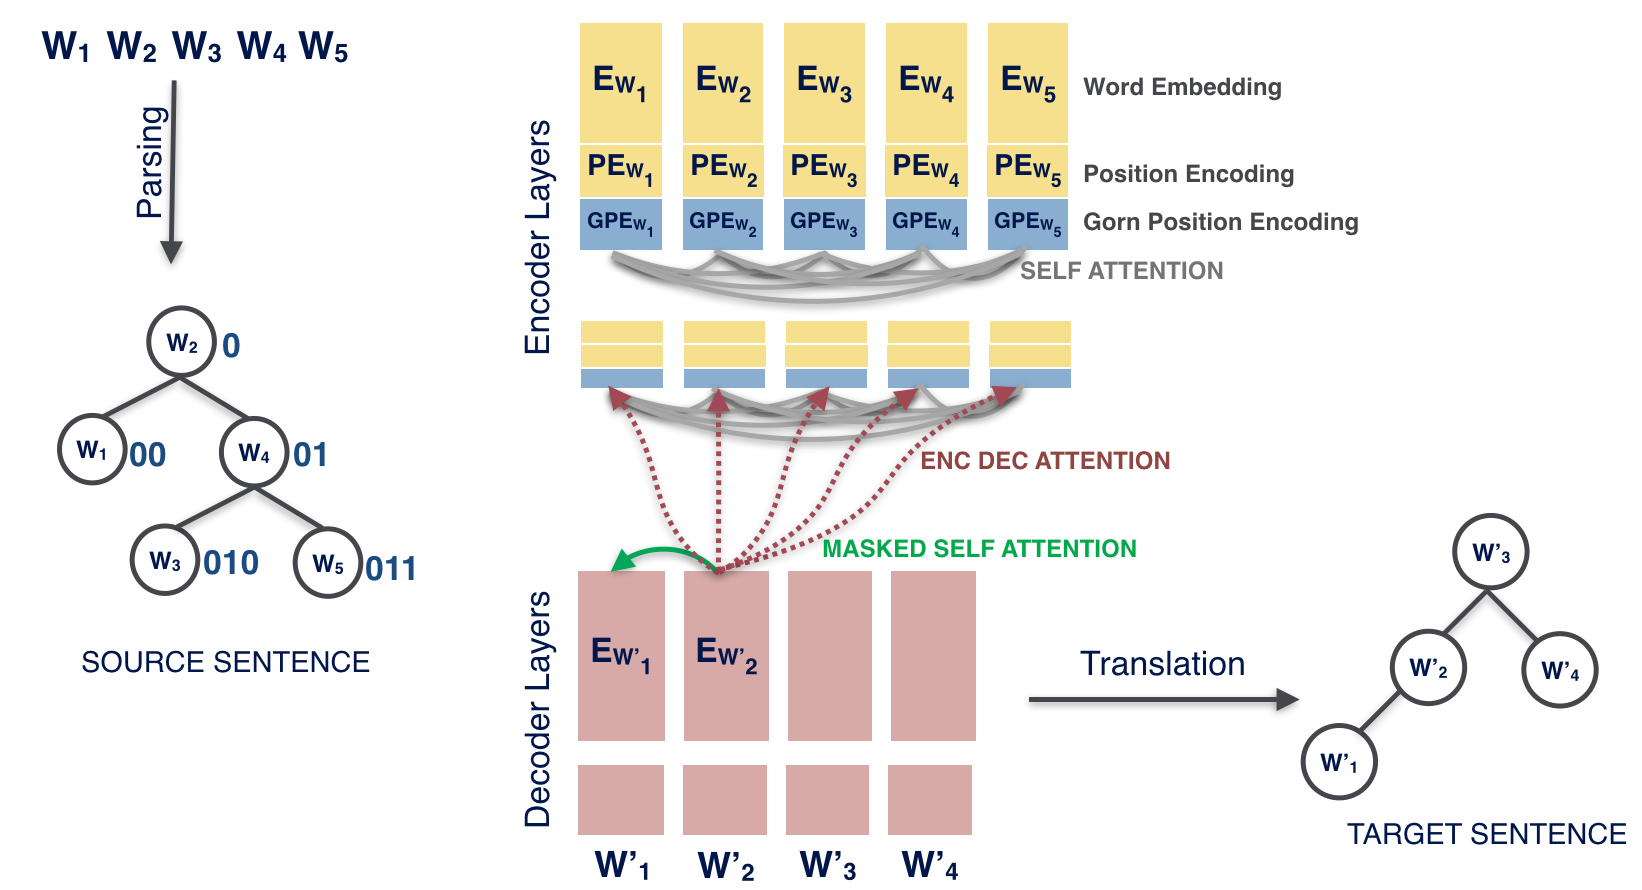
\includegraphics[width=13cm]{pictures/Architecture.png}
    \caption{High Level Architecture}
    \label{fig:architecture}
\end{figure}

The transformer model does not any form of contain recurrence or convolution, the approaches that inject the order of the sequence to the model. So, in order to make the model aware of the sequence, positional encoding tokens - which correspond to the absolute position of the tokens in the sequence, are added to the word embeddings. We extended this approach, to further incorporate the Gorn Position Encoding in the input representation and employed following different ways to do it:

\\
\textbf{Gorn Address Addition} - The positional encodings in the transformer model have the same number of dimensions as the embeddings and each dimension corresponds to a sinusoid. Positional Embeddings and Word Embeddings are then summed together to get the final embeddings. We followed the same procedure for Gorn Position Embeddings and calculated the corresponding sinusoid based gorn Position Embeddings and added it to the previous embedding. We experimented with a few variations such as cosine for odd dimensions and sine for even vs sine for odd and cosine for even. But the performance of the model deteriorated by this addition seemingly due to the confusion created by summing Positional Encoding and Gorn Positional Encoding and not providing any clear distinction between the two.

\\
 \textbf{Gorn Address Concatenation} - We then concatenated Positional Encoding and Gorn Positional Encoding rather than adding them. To avoid increasing the number of model parameters, we provided the Positional Encoding information in half of the dimensions as the word embeddings and Gorn Positional Encoding in the other half. This setting gave interesting insights and better performance in a most of the tasks when compared to the models with no syntactic information. Whereas, the sequence with attention and transformer models having explicit syntactic information performed better than this model. 
 
\\
\textbf{Relative Position Representation}
Recent work by \citet{Shaw2018SelfAttentionWR} presented an alternative way of encoding position information as relative rather than absolute as discussed in \citet{Vaswani2017AttentionIA}. The paper mentions that the proposed self-attention mechanism has the potential to generalize to arbitrary graph labeled inputs and shows promising results on machine translation task. We augmented their model of adding relative sequence ordering to incorporate the syntactic structure in the input representation. We added simplified graph structure(a tree) by including relative parent, relative sibling and relative children distances to the model.

\section{Experiments}\label{Experiments}
\subsection{Synthetic Tasks}
To train and evaluate our framework, we designed a set of intrinsic tasks that closely map with the tasks in natural language processing - Simple Node Relabeling, Complex Node Relabeling, Tree Reordering and Subtree Deletion. Refer \autoref{fig:tree_simple_relabel} for illustration. 
%\begin{wrapfigure}{R}{0.5\textwidth}
\begin{figure}
\centering
\resizebox{0.45\textwidth}{!}{%
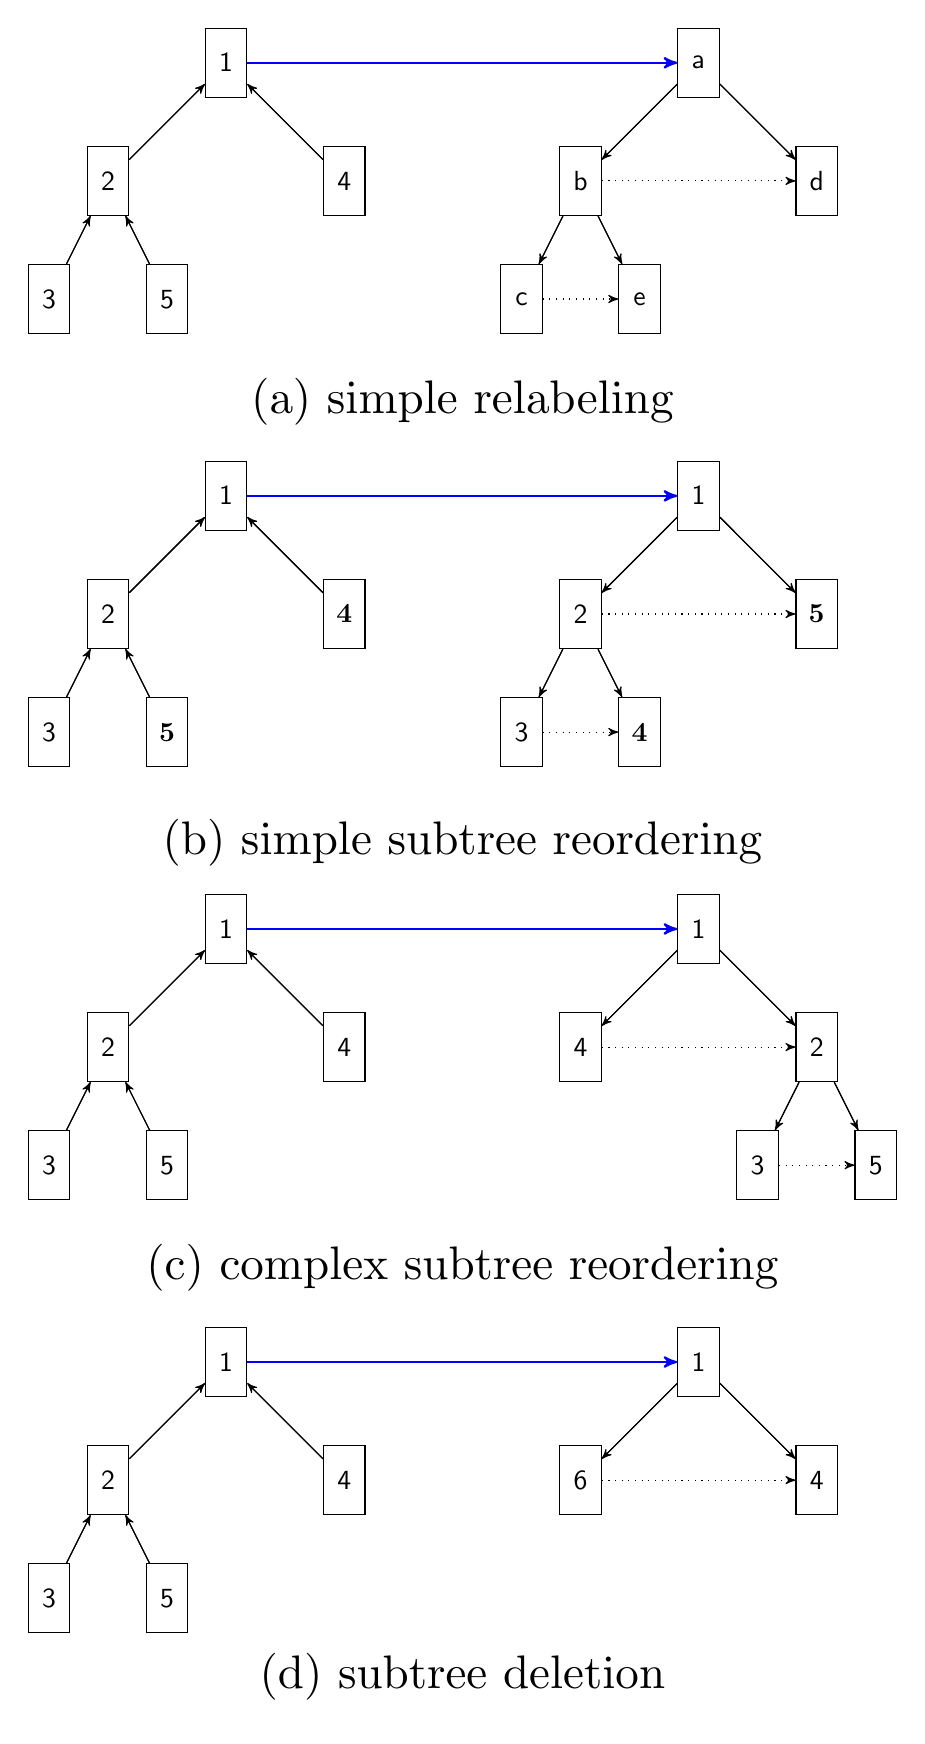
\begin{tikzpicture}[-,>=stealth',level/.style={sibling distance = 3cm/#1,
  level distance = 1.5cm}] 
    \node (S) [arn_x]  at (-3, 16.5) {1}
    child{ node (2) [arn_x] {2}
        child{ node (3) [arn_x] {3}}
        child{ node (4) [arn_x] {5}}
    }
    child{ node (5) [arn_x] {4}}
;
% 
    \node (T) [arn_x] at (3, 16.5) {a}{
        child{ node (b) [arn_x] {b}
            child{ node (c) [arn_x] {c}}
            child{ node (d) [arn_x] {e}}
        }
        child{ node (e) [arn_x] {d}}}
    ;    
\draw[->,thick,blue] (S) edge (T);   
\draw[->] (3) edge (2);   
\draw[->] (4) edge (2);   
\draw[->] (2) edge (S);   
\draw[->] (5) edge (S);
%
\draw[->] (T) edge (b);   
\draw[->] (b) edge (c);   
\draw[->] (b) edge (d);
\draw[->, dotted] (c) edge (d);
\draw[->] (T) edge (e);   
\draw[->, dotted ] (b) edge (e);
%
%
\node[scale=1.7] at (0,12.2) { (a) simple relabeling };
%
%
    \node (RLS) [arn_x]  at (-3, 11) {1}
    child{ node (RL2) [arn_x] {2}
        child{ node (RL3) [arn_x] {3}}
        child{ node (RL4) [arn_x] {{\bf 5}}}
    }
    child{ node (RL5) [arn_x] {{\bf 4}}}
;
% 
    \node (RLT) [arn_x] at (3,11) {1}{
        child{ node (RLb) [arn_x] {2}
            child{ node (RLc) [arn_x] {3}}
            child{ node (RLd) [arn_x] {{\bf 4}}}
        }
        child{ node (RLe) [arn_x] {{\bf 5}}}}
    ;    
\draw[->,thick,blue] (RLS) edge (RLT);   
\draw[->] (RL3) edge (RL2);   
\draw[->] (RL4) edge (RL2);   
\draw[->] (RL2) edge (RLS);   
\draw[->] (RL5) edge (RLS);
%
\draw[->] (RLT) edge (RLb);   
\draw[->] (RLb) edge (RLc);   
\draw[->] (RLb) edge (RLd);
\draw[->, dotted] (RLc) edge (RLd);
\draw[->] (RLT) edge (RLe);   
\draw[->, dotted ] (RLb) edge (RLe);
%
%
\node[scale=1.7] at (0,6.6) {(b) simple subtree reordering};
%
%
    \node (ROS) [arn_x]  at (-3, 5.5) {1}
    child{ node (RO2) [arn_x] {2}
        child{ node (RO3) [arn_x] {3}}
        child{ node (RO4) [arn_x] {5}}
    }
    child{ node (RO5) [arn_x] {4}}
;
% 
    \node (ROT) [arn_x] at (3,5.5) {1}{
        child{ node (ROe) [arn_x] {4}}
        child{ node (ROb) [arn_x] {2}
            child{ node (ROc) [arn_x] {3}}
            child{ node (ROd) [arn_x] {5}}
        }
        }
    ;    
\draw[->,thick,blue] (ROS) edge (ROT);   
\draw[->] (RO3) edge (RO2);   
\draw[->] (RO4) edge (RO2);   
\draw[->] (RO2) edge (ROS);   
\draw[->] (RO5) edge (ROS);
%
\draw[->] (ROT) edge (ROb);   
\draw[->] (ROb) edge (ROc);   
\draw[->] (ROb) edge (ROd);
\draw[->, dotted] (ROc) edge (ROd);
\draw[->] (ROT) edge (ROe);   
\draw[->, dotted ] (ROe) edge (ROb);
%
%
\node[scale=1.7] at (0,1.2) {(c) complex subtree reordering};
%
%
    \node (DS) [arn_x]  at (-3, 0) {1}
    child{ node (D2) [arn_x] {2}
        child{ node (D3) [arn_x] {3}}
        child{ node (D4) [arn_x] {5}}
    }
    child{ node (D5) [arn_x] {4}}
;
% 
    \node (DT) [arn_x] at (3,0) {1}{
        child{ node (Db) [arn_x] {6}
        }
        child{ node (De) [arn_x] {4}}}
    ;    
\draw[->,thick,blue] (DS) edge (DT);   
\draw[->] (D3) edge (D2);   
\draw[->] (D4) edge (D2);   
\draw[->] (D2) edge (DS);   
\draw[->] (D5) edge (DS);
%
\draw[->] (DT) edge (Db);   
\draw[->] (DT) edge (De);   
\draw[->, dotted ] (Db) edge (De);

\node[scale=1.7] at (0,-4.0) {(d) subtree deletion};


\end{tikzpicture}
}
\caption{a) Simple relabeling example where $1 \rightarrow a$, $2 \rightarrow b$, and so on. b) subtree reordering where nodes labeled 4 and 5 swap. c) full reordering of subtree where left and right subtrees of the root node swap, and d) subtree deletion where the subtree of node 2 is replaced be the node labelled 6. The dotted arrows represent conditional dependence.} \label{fig:tree_simple_relabel}
\end{figure}

%\end{wrapfigure}



\subsection{Data Preparation}
To prepare data for these synthetic tasks, we designed deterministic context aware tree transduction rules. Then, we generated common set of trees with a maximum depth of 7 and a vocabulary size of 256 with internal nodes in the range of [0-10]. These trees were then passed through the four set of rules to yield the valid input and output trees. We then split this data into training, validation and test sets. \par
Post raw data creation, we enriched both the source and target trees with the corresponding gorn addresses. We experimented with both sequence and tree based learning for these tasks. \autoref{tab: input-representation} shows the models and task variants employed for each intrinsic task along with the corresponding input representations for the sample tree in \autoref{fig: example-binary-tree}.

\newfloatcommand{capbtabbox}{table}[][\FBwidth]
\begin{figure}[H]
\begin{floatrow}
\ffigbox{
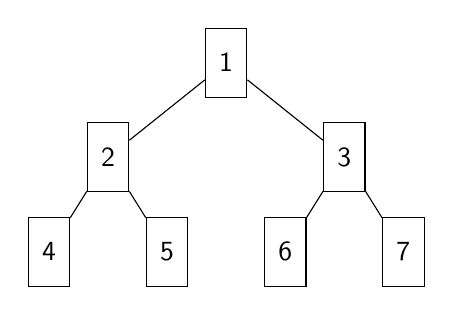
\begin{tikzpicture}[-,>=stealth',level/.style={sibling distance = 3cm/#1,  level distance = 1.2cm}] 
% \node [arn_x] {\ \ (a + b) $*$ c \ \ }
     \node [arn_x] {1}
        child{ node [arn_x] {2}
            child{ node [arn_x] {4}}
            child{ node [arn_x] {5}}
        }
        child{ node [arn_x] {3}
            child{ node [arn_x] {6}}
            child{ node [arn_x] {7}}
        }
    ;
\end{tikzpicture}
}{%
  \caption{Example binary tree -  4 2 5 1 6 3 7}%
  \label{fig: example-binary-tree}
}


\capbtabbox{%
    \def\arraystretch{1.15}
   \begin{tabular}{|c|c|c|}
\hline
\textbf{Task} & \textbf{Model} & \textbf{Input Representation} \\ \hline
\multirow{3}{*}{SEQ} & Seq2Seq & 4 2 5 1 6 3 7 \\ \cline{2-3} 
 & Transformer & \begin{tabular}[c]{@{}c@{}}4 2 5 1 6 3 7\\ 1 2 3 4 5 6 7\end{tabular} \\ \cline{2-3} 
 & Trans+Gorn & \begin{tabular}[c]{@{}c@{}}4 2 5 1 6 3 7\\ 1 2 3 4 5 67\\ 4 2 5 1 6 3 7\end{tabular} \\ \hline
\multirow{3}{*}{TREE} & Seq2Seq & ( 1 ( 2 4 5 ) ( 3 6 7 ) ) \\ \cline{2-3} 
 & Transformer & \begin{tabular}[c]{@{}c@{}}(  1 ( 2 4 5  ) (  3  6   7   )   )\\ 1 2 3 4 5 6 7 8 9 10 11 12 13\end{tabular} \\ \cline{2-3} 
 & Trans+Gorn & \begin{tabular}[c]{@{}c@{}}1 2 4 5 3 6 7\\ 4 2 1 3 6 5 7\\ 1 2 3 4 5 6 7\end{tabular} \\ \hline
\end{tabular}
}{%
%   \caption{A table}%
  \caption{Sample Input representation}%
  \label{tab: input-representation}
}
\end{floatrow}
\end{figure}




\subsection{Evaluation}
We evaluated a set of different methods using Tree Edit Distance - TED \citep{bille2005survey}, between the predicted tree and the actual tree. TED is the number of insertions, deletions, and modifications to make the two trees equivalent, while aligning the trees. To understand the difficulty of the tasks, we calculated the TED between the input and output trees for all tasks which is: 8 for Simple Relabeling, 6 for Complex Relabeling, 18 for Reordering and 14 for Deletion.

\section{Results and Analysis}
\autoref{fig:deletion}, \autoref{fig:relabeling} and \autoref{fig:reordering} show the training and validation ac-curacies of six variants each on Deletion, Relabeling and Reordering tasks respectively. Three (Labels starting with SEQ in the plots; the ones with solid lines) of the six variants are provided with only sequence/surface level information. Whereas, the other three (Labels starting with TREE in the plots; the ones with dotted lines) are additionally provided with explicit syntactic information. 
\begin{figure}[H]
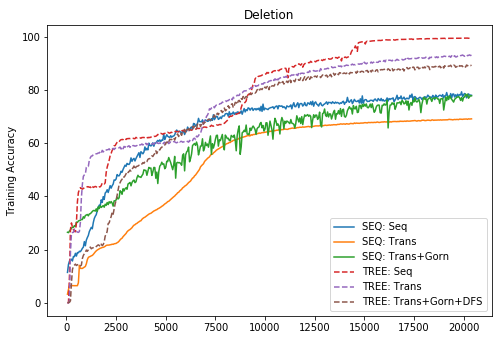
\includegraphics[width=6.5cm]{pictures/Deletion_Training.png}
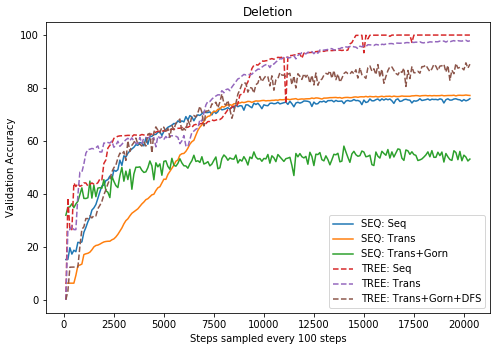
\includegraphics[width=6.5cm]{pictures/Deletion_Validation.png}
    \caption{Training and Validation Accuracy with steps for Deletion}
    \label{fig:deletion}
\end{figure}
\begin{figure}[H]
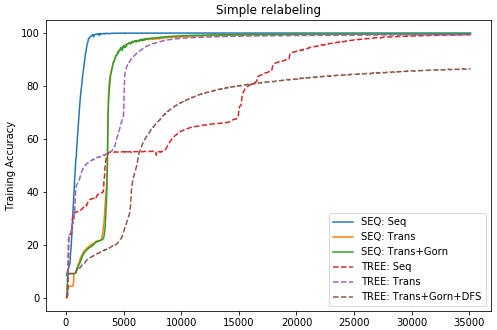
\includegraphics[width=6.5cm]{pictures/Simple_Training.png}
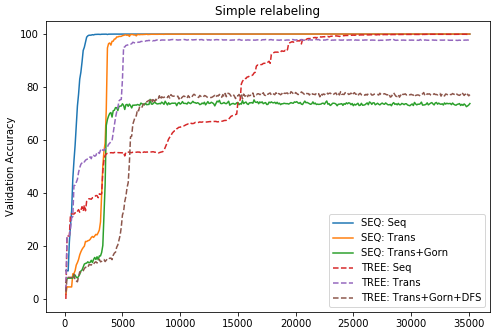
\includegraphics[width=6.5cm]{pictures/Simple_Validation.png}
    \caption{Training and Validation Accuracy with steps for Simple Relabeling}
    \label{fig:relabeling}
\end{figure}

\begin{figure}[H]
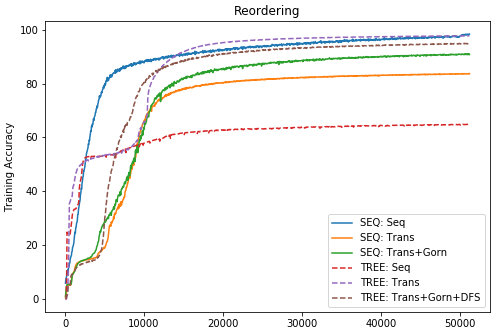
\includegraphics[width=6.5cm]{pictures/Reordering_Validation.png}
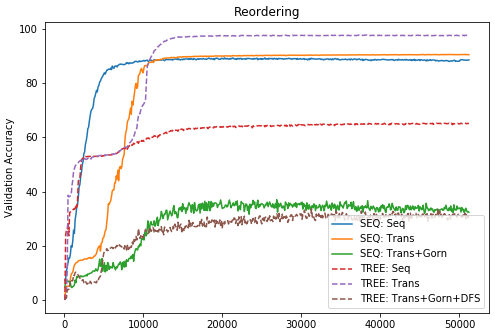
\includegraphics[width=6.5cm]{pictures/Reordering_Training.png}
    \caption{Training and Validation Accuracy with steps for Reordering}
    \label{fig:reordering}
\end{figure}

For simple tasks - the ones not requiring enough contextual information such as Simple Relabeling (\autoref{fig:relabeling}), extra syntactic information doesn't help in-fact it slows down the learning process. But eventually both models reach more than 99 \% accuracy. \par
On the other hand, for complex tasks such as Deletion, it is evident from the plots (\autoref{fig:deletion}) that all models with syntactic information are performing better than the ones without it corroborating the fact that explicit transduction step helps the model to learn better. \par
It is also interesting to note from the gap between the training and validation accuracies of all three tasks that the models with gorn address are overfitting which hints that Gorn is allowing the model to cheat. Also, tuning dropout didn't help in improving the validation accuracy.



% \todo{Add Plots here}
% \section{Conclusion}
\bibliography{t2t_tranformer}
\bibliographystyle{act_natbib}
\end{document}